\chapter{Implementation} \label{chap:implementation}

\section*{}

\begin{Notes}
- Talk about iRAP configuration, the result combination tool and more.\\
- Talk about PBS Finder configuration, requisites and analysis flow (show that analysis flow diagram).\\
- Talk about platform extensibility, deployment alternatives and more.\\
\end{Notes}

\section{Gene Expression Analysis Pipeline}

\section{RNA Binding Protein Analysis Web Platform}

\subsection{Application Structure}

\subsubsection*{Configuration}

\subsection{Analysis Workflow}

\begin{figure}[!htb]
  \begin{center}
    \leavevmode
    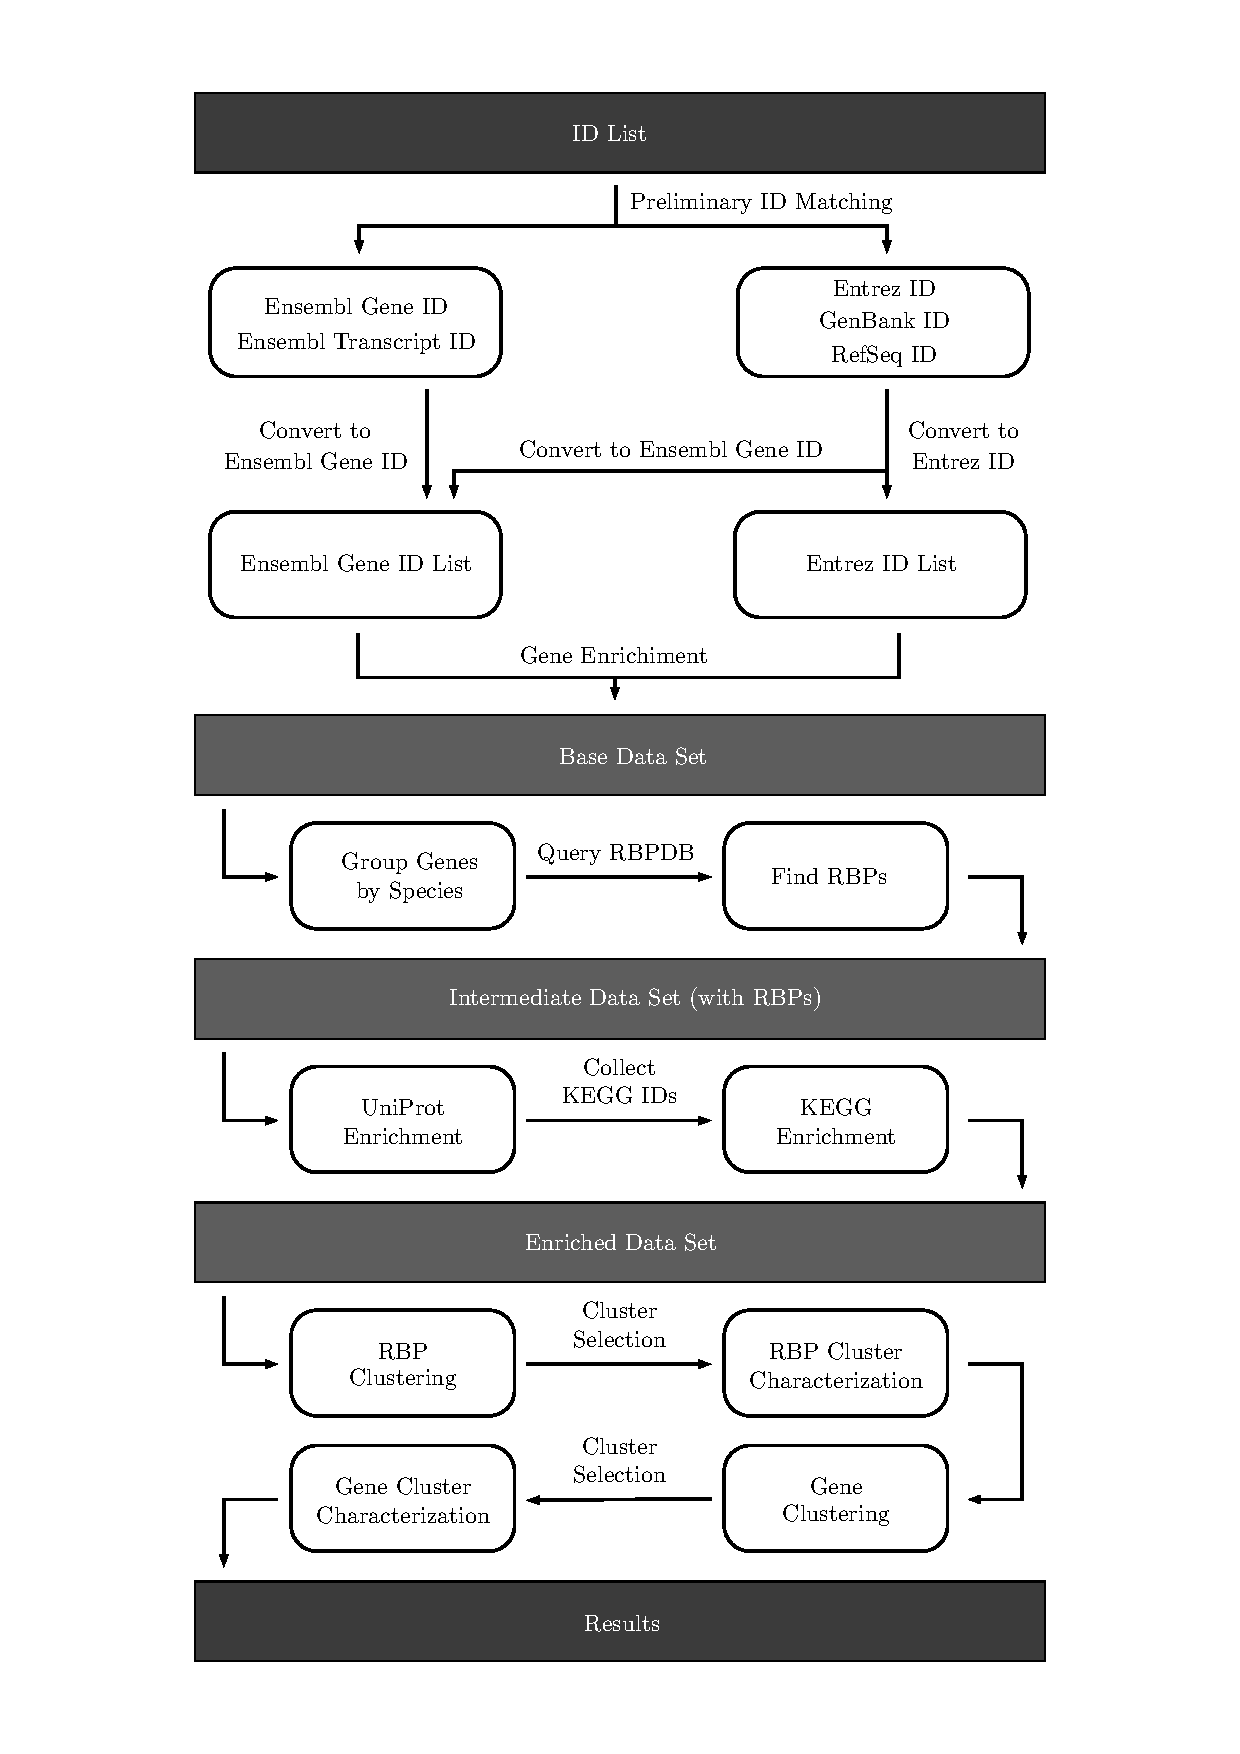
\includegraphics[width=0.75\textwidth]{workflow}
    \caption[PBS Finder workflow]{
      PBS Finder workflow. Note that error paths were not represented for
      simplicity. However, every component implements health checks, that may
      stop the entire analysis if the minimum requirements for success are not
      met.
    }
    \label{fig:workflow}
  \end{center}
\end{figure}

\subsection{Data Set Enrichment}

\subsection{Clustering Analysis}

\subsubsection*{ILP Clustering}

\subsection{Web Interface}

\subsubsection*{Job View}

\subsubsection*{Transcript View}

\subsubsection*{Protein View}

\subsubsection*{Results Exporting}

\section{Deployment}

\section{Chapter Conclusions}

